\definecolor{exxetagray}{gray}{0.75}
\definecolor{itemcolor}{RGB}{179,217,255}
\definecolor{usercolor}{RGB}{255,204,179}

\shorthandoff{"}
\chapter{Diskussion}
\label{ch:diskussion}

\section{Zusammenfassung der Ergebnisse}
Im Rahmen der quantitativen Forschung dieser Arbeit wurde untersucht, ob der entwickelte multi-kriterielle Ansatz für die Berücksichtigung der Präferenzen in einem bilateralen Empfehlungssystem, robust die Zufriedenheit von Mitarbeitenden erhöhen kann, ohne Einbußen in der zu erwartenden Arbeitsleistung der Mitarbeitenden bei der Besetzung von offenen Projektpositionen zu bewirken.
Anhand einer Befragung unter den Mitarbeitenden des IT-Unternehmens EXXETA wurden Fähigkeiten und Präferenzen von Mitarbeitenden sowie deren Zufriedenheit mit ausgewählten Beispielprojekten ermittelt.
Eine Befragung unter den Managern desselbigen Unternehmens diente dazu, die zu erwartende Arbeitsleistung der befragten Mitarbeitenden in den ausgewählten Projekten zu bestimmen.
Die Zufriedenheit und die zu erwartende Arbeitsleistung wurde jeweils für die empfohlenen Mitarbeitenden des unilateralen sowie die empfohlenen Mitarbeitenden des bilateralen Systems gemessen und miteinander verglichen.
Insgesamt konnte festgestellt werden, dass der bilaterale Algorithmus im Mittel in vier von fünf Projekten eine höhere Zufriedenheit erzielte und in zwei der fünf Projekte eine Steigerung der Arbeitsleistung bewirkte.
Dabei führte der bilaterale Algorithmus in 28 Prozent der Fälle zu einer erhöhten Zufriedenheit unter den empfohlenen Mitarbeitenden und in 20 Prozent der Fällen zu einer Steigerung der prognostizierten Arbeitsleistung der empfohlenen Mitarbeitenden.
Zugleich führte der bilaterale Algorithmus in 12 Prozent der Fälle zu einer Verschlechterung der erwarteten Arbeitsleistung.
Der Rückgang der Arbeitsleistung konnte zwei der fünf Projekte zugeordnet werden.
Lediglich in 8 Prozent der Fälle bewirkte der bilaterale Algorithmus einen Rückgang der Zufriedenheit unter den empfohlenen Mitarbeitenden.
Die Verschlechterung der Zufriedenheit wurde genau in einem der fünf Projekte bewirkt.
% In 12 Prozent der Fälle führte der bilaterale Algorithmus dagegen zu einer Verschlechterung der zu erwartenden Arbeitsleistung.
% In 8 Prozent der Fälle bewirkte der bilaterale Algorithmus sogar eine Verschlechterung der Zufriedenheit unter den empfohlenen Mitarbeitenden.

% Kurz eingehen auf die ergebnisse der präferenz und fähigkeitsbefragung
Bei der Befragung der Mitarbeitenden zu ihren Fähigkeiten und Präferenzen konnte festgestellt werden, dass Mitarbeitende den Großteil der angefragten Fähigkeiten präferierten, während sie nahezu gleich vielen angeforderten Fähigkeiten neutral gegenüber standen.
Weiter wurde sichtbar, dass der Großteil der Fähigkeiten von Mitarbeitenden sowohl beherrscht als auch präferiert wurde.
Durch die Integration der negativen Präferenzen wurde sichtbar, dass Mitarbeitende bei über 22 Prozent der angeforderten Fähigkeiten kein Interesse zeigten diese in zukünftigen Projekten einsetzen zu wollen.
Ein Vergleich der Erfüllung der Präferenzen der Mitarbeitenden durch die angeforderten Projektpositionen und deren Zufriedenheit in den jeweiligen Projekten zeigte darüber hinaus bei zwei der fünf Beispielprojekte eine auffällige Diskrepanz.

Die Befragung der Manager legte offen, dass deren Angaben zu der prognostizierten Arbeitsleistung der Mitarbeitenden in den ausgewählten Projekten bei zwei der Beispielprojekte auffällig auseinanderfielen. 
Ein Vergleich der Erfüllung der angeforderten Projektpositionen durch die Mitarbeitenden und deren erwarteter Arbeitsleistung nach Angaben der Manager zeigte darüber hinaus, dass die angegebenen Mitarbeitenden in einigen Projekten nicht konkruent mit den Mitarbeitenden mit der höchsten Erfüllung der angeforderten Projektpositionen waren.

Abschließend wurde betrachet, wie sich die Gewichtung von Fähigkeiten und Präferenzen auf die Zufriedenheit und die Arbeitsleistung der Mitarbeitenden auswirkte.
Dabei wurde festgestellt, dass die Methode zur Bestimmung des optimalen Gewichts bei unterschiedlichen Kombinationen der Traningsdatensätze zu Gewichten führte, die alle in einen Bereich zwischen 0.6 und 0.8 fielen.
Bei Betrachtung der Zufriedenheit und der Arbeitsleistung unter Anwendung der verschiedenen Gewichte fiel auf, dass die Steigerung der Zufriedenheit und der Arbeitsleistung durch kein bestimmtes Gewicht erzielt wurde.
Auch die Fälle, die eine Verschlechterung der Zufriedenheit bzw. der Arbeitsleistung aufwiesen konnten nicht gezielt einem Gewicht zugeordnet werden.

\section{Interpretation der Ergebnisse}
Basierend auf den Forschungsergebnissen von \textcite[S.1 ff.]{link:booklet} wurde die Annahme aufgestellt, dass ein alternativer Ansatz für die Berücksichtigung der Präferenzen beider Parteien in einem bilateralen Empfehlungssystems robust zu einer verbesserten Zuordnung von Person zu Umgebung im Vergleich zu einem unilateralen System führen kann.
% Als Indikatoren einer optimalen Zuordnung betrachtete \textcite[S.1 ff.]{link:booklet} die Kennzahlen Zufriedenheit und Arbeitsleistung.
Die Ergebnisse der quantitativen Forschung zeigen, dass der entwickelte multi-kriterielle Ansatz für das bilaterale Empfehlungssystem verglichen mit dem unilateralen System in vier von fünf Projekten im Mittel eine höhere Zufriedenheit unter den empfohlenen Mitarbeitenden erzielen konnte (Vgl. Abbildung \ref{fig:ergebnisse:abb8}).
Zugleich blieb die Arbeitsleistung in drei von fünf Projekten im Mittel konstant, wobei in zwei der fünf Projekte durchschnittlich sogar eine Steigerung der Arbeitsleistung unter Einsatz des bilateralen Algorithmus erzielt wurde (Vgl. Abbildung \ref{fig:ergebnisse:abb10}).
Insgesammt lassen die Auswirkungen des entwickelten bilateralen Algorithmus auf die durchschnittliche Zufriedenheit und Arbeitsleistung der Mitarbeitenden daher die Vermutung zu, dass eine Berücksichtigung der Präferenzen grundsätzlich vorteilhaft ist.

Entgegen der Erwartungen bewirkte der bilaterale Algorithmus in zwei von 25 Fällen eine Verschlechterung der Zufriedenheit unter den empfohlenen Mitarbeitenden (Vgl. Abbildung \ref{fig:ergebnisse:abb9}).
Ein Vergleich der unilateralen und bilateralen Rankings zeigte, dass die Verschlechterung der Zufriedenheit in beiden Fällen durch denselben Mitarbeitenden in Projekt 3 bewirkt wurde.
Tabelle \ref{tab:diskussion:tab1} stellt für einen der Fälle ($\alpha$ = 0.6068) das unilaterale Top-5-Ranking im Vergleich zu den Rängen der Mitarbeitenden im bilateralen Ranking dar.

\begin{table}[htbp]
    \begin{center}
    \begin{tabular}{c|p{0.7in}|p{0.7in}|p{0.7in}|p{0.7in}}
    {\textbf{Mitarbeitender}} & {\textbf{Rang unilateral}} & {\textbf{Rangwert unilateral}} & {\textbf{Rang bilateral}} & {\textbf{Rangwert bilateral}} \\
    \hline
	Mitarbeitender A & \hfil1 & \hfil0.625 & \hfil3 & \hfil0.5759 \\
    \hline
    Mitarbeitender B & \hfil2 & \hfil0.625 & \hfil5 & \hfil0.5513 \\
    \hline
	Mitarbeitender C & \hfil3 & \hfil0.625 & \hfil6 & \hfil0.5514 \\
    \hline
	Mitarbeitender D & \hfil4 & \hfil0.625 & \hfil2 & \hfil0.6004 \\
    \hline
	Mitarbeitender E & \hfil5 & \hfil0.5625 & \hfil1 & \hfil0.6362 \\
    \end{tabular}
    \end{center}
    \caption[Vergleich des unilateralen Top-5-Rankings mit den bilateralen Rängen der empfohlenen Mitarbeitenden für Projekt 3 ($\alpha$ = 0.6068)]{Vergleich des unilateralen Top-5-Rankings mit den bilateralen Rängen der empfohlenen Mitarbeitenden für Projekt 3 ($\alpha$ = 0.6068)}
	\label{tab:diskussion:tab1}
\end{table}

Daran ist zu erkennen, dass der Mitarbeitende C durch die Berücksichtigung der Präferenzen im bilateralen Ranking auf Rang 6 platziert wurde und damit nicht mehr unter die fünf empfohlenen Mitarbeitenden fiel.
% Der Mitarbeitende wurde aufgrund seiner geringen Übereinstimmung der angegebenen Präferenzen mit den angeforderten Projektpositionen von Projekt 3 im bilateralen Ranking niedriger platziert als im unilateralen Ranking.
Obwohl der Mitarbeitende die Mehrheit der angeforderten Fähigkeiten des Projekts nicht präferierte, konnte festgestellt werden, dass dieser in der Befragung dennoch angab mit dem Projekt grundsätzlich zufrieden zu sein.
Die geringere Zufriedenheit bei bilateraler Empfehlung wurde folglich durch eine niedrigere Platzierung des Mitarbeitenden aufgrund der hohen Gewichtung der Präferenzen im Vergleich zum unilateralen Ranking bewirkt.
Der Sachverhalt lässt vermuten, dass neben den Präferenzen eines Mitarbeitenden offenbar weitere unbekannte Faktoren existieren, die die Zufriedenheit eines Mitarbeitenden beeinflussen.
Eine Annahme ist, dass unterschiedliche Fähigkeiten in Projekten von unterschiedlicher Bedeutung für einen Mitarbeitenden sind.
Es wird vermutet, dass das Vorhandensein oder Fehlen bestimmter Projektposition in einem Projekt ausschlaggebend für die Zufriedenheit eines Mitarbeitenden in einem Projekt sein kann, unabhängig von dessen übrigen Präferenzangaben.

In Kapitel ...AUF KAPITEL 5 METHODIK VERWEISEN...  wurde angeführt, dass die Berücksichtigung der Zufriedenheit der Mitarbeitenden bei der Zuordnung zu Projekten mit deren erwarteter Arbeitsleistung in Projekten in Konkurrenz stehen kann.
Es wurde daher durchaus erwartet, dass die Berücksichtigung der Zufriedenheit der Mitarbeitenden in einigen Fällen auch zu einer Reduktion der erwarteten Arbeitsleistung führen würde.
Die absolute Veränderung der Arbeitsleistung der Mitarbeitenden von unilateralem zu bilateralem Algorithmus nach Projekt in Abbildung \ref{fig:ergebnisse:abb11} zeigte, dass dies in drei von 25 Fällen auftrat.
Tabelle \ref{tab:diskussion:tab2} stellt für einen der Fälle (Projekt 2, $\alpha$ = 0.6068) das unilaterale Top-6-Ranking im Vergleich zu den Rängen der Mitarbeitenden im bilateralen Ranking dar.

\begin{table}[htbp]
    \begin{center}
    \begin{tabular}{c|p{0.7in}|p{0.7in}|p{0.7in}|p{0.7in}}
    {\textbf{Mitarbeitender}} & {\textbf{Rang unilateral}} & {\textbf{Rangwert unilateral}} & {\textbf{Rang bilateral}} & {\textbf{Rangwert bilateral}} \\
    \hline
	Mitarbeitender A & \hfil1 & \hfil0.875 & \hfil3 & \hfil0.7767 \\
    \hline
    Mitarbeitender B & \hfil2 & \hfil0.8125 & \hfil1 & \hfil0.8862 \\
    \hline
	Mitarbeitender C & \hfil3 & \hfil0.75 & \hfil2 & \hfil0.7992 \\
    \hline
	Mitarbeitender D & \hfil4 & \hfil0.5 & \hfil4 & \hfil0.6720 \\
    \hline
	Mitarbeitender E & \hfil5 & \hfil0.375 & \hfil6 & \hfil0.4979 \\
    \hline
	Mitarbeitender F & \hfil6 & \hfil0.375 & \hfil5 & \hfil0.5225 \\
    \end{tabular}
    \end{center}
    \caption[Vergleich des unilateralen Top-6-Rankings mit den bilateralen Rängen der empfohlenen Mitarbeitenden für Projekt 2 ($\alpha$ = 0.6068)]{Vergleich des unilateralen Top-6-Rankings mit den bilateralen Rängen der empfohlenen Mitarbeitenden für Projekt 2 ($\alpha$ = 0.6068)}
	\label{tab:diskussion:tab2}
\end{table}

Bei näherer Betrachtung der unilateralen und bilateralen Rankings fällt auf, dass Mitarbeitender E und F im unilateralen Ranking denselben Rangwert aufwiesen.
Durch die Berücksichtigung der Präferenzen rückte der Mitarbeitende F im bilateralen Ranking vor den Mitarbeitenden E, wodurch dieser nicht unter die empfohlenen Personen des bilateralen Rankings fiel.
Auffällig ist, dass beide Mitarbeitende im unilateralen Ranking denselben Rangwert aufwiesen.
Entgegen der Erwartungen zeigte ein Vergleich der Angaben der Manager zu der erwarteten Arbeitsleistung der Mitarbeitenden in Projekt 2 jedoch, dass lediglich von dem Mitarbeitenden E eine hohe Arbeitsleistung erwartet wurde.
Dies lässt die Vermutung zu, dass neben den Fähigkeiten weitere Faktoren die Auswahl der Manager bei der Zuordnung von Mitarbeitenden für offene Projekte beeinflussen.
Eine Vermutung ist, dass auch bei der Besetzung von Projekten mit Mitarbeitenden das Vorhandensein bzw. Fehlen spezifischer Fähigkeiten der Mitarbeitenden ausschlaggebend für die Zuordnung durch die Manager sein kann.  
Es wird angenommen, dass die Auswahl der Manager möglicherweise dadurch beeinflusst wird, wie schnell Mitarbeitende basierend auf ihren vorhanden Fähigkeiten projektkritische Fähigkeiten erlernen können.

% - interpretation von zufriedenheit und arbeitsleistung insgesamt und ausreisser erklären mit bezug zu kapitel 3, wo erklärt wird, dass man präferenzen integrieren soll

% Die in Kapitel .. vorgestellten verwandten Arbeiten über die Kombination der Präferenzen zweier Parteien in einem Empfehlungssystem ließen vermuten, dass die unterschiedliche Gewichtung der Präferenzen

Die Ergebnisse der Arbeiten von \textcite[S. 131ff.]{kleinerman:2:inproceedings} und \textcite[S. 4031 ff.]{neve:inproceedings} ließen darüber hinaus erwarten, dass eine individuelle Gewichtung der Präferenzen beider Parteien eines Empfehlungssystems die Qualität der Empfehlungen positiv beeinflussen kann.
% In Kapitel \ref{ch:verwandte_arbeiten} wurde im Rahmen der verwandten Arbeiten angeführt, dass eine Gewichtung der Präferenzen beider Parteien eines Empfehlungssystems die Qualität der Empfehlungen positiv beeinflussen kann.
Aufgrund der Natur des Anwendungsfalls wurde angenommen, dass eine geringere Gewichtung der Fähigkeiten ($\alpha$ <= 0.5) und die damit einhergehende höhere Gewichtung der Präferenzen in einer höheren Zufriedenheit und niedrigeren Arbeitsleistung unter den empfohlenen Mitarbeitenden resultiert.
Zugleich wurde erwartet, dass eine höhere Gewichtung der Fähigkeiten ($\alpha$ > 0.5) und die damit einhergehende geringere Gewichtung der Präferenzen eine höhere Arbeitsleistung sowie eine niedrigere Zufriedenheit bewirken.
Die Ergebnisse der Fallstudie zeigten jedoch keinen eindeutigen Trend hinsichtlich Zufriedenheit und Arbeitsleistung bei unterschiedlicher Gewichtung der Fähigkeiten und Präferenzen.
Dies ist daran zu erkennen, dass die Verschlechterung bzw. Verbesserung von weder Zufriedenheit noch Arbeitsleistung eindeutig bestimmten Gewichten zugeordnet werden kann (Vgl. Abbildung \ref{fig:ergebnisse:abb12} und Abbildung \ref{fig:ergebnisse:abb13}).

Eine Vermutung für den unklaren Trend lag darin, dass die untersuchten $\alpha$-Werte für die Menge der vorhanden Daten (13 Mitarbeitende je Gewicht) zu nah beieinander lagen.
Daher wurde der bilaterale Algorithmus anhand der gesamten Daten (54 Mitarbeitende) für Grenzfälle von $\alpha$ evaluiert, einmal mit $\alpha$ = 0.1 und einmal mit $\alpha$ = 0.9 als Gewicht.
Die Ergebnisse sind in Abbildung \ref{fig:diskussion:abb1} dargestellt.

\begin{figure}[H]
    \centering
	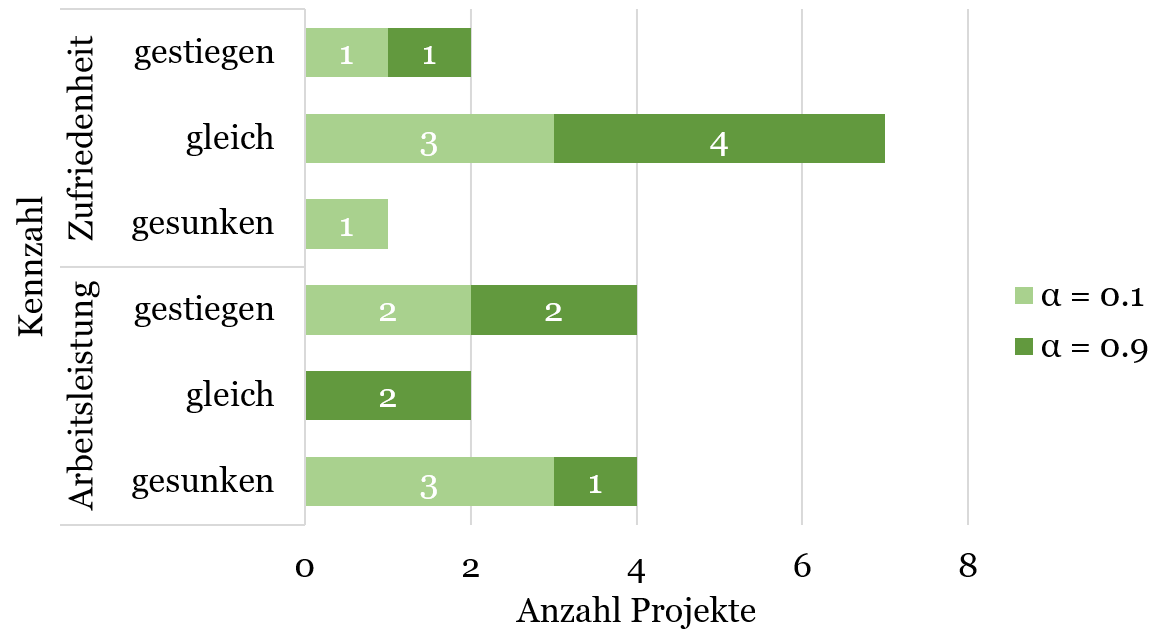
\includegraphics[width=0.95\textwidth]{gfx/verhaeltnis-z-a-projekte-edge-cases.png}
	\caption[Veränderung von Zufriedenheit und Arbeitsleistung der Mitarbeitenden von unilateralem zu bilateralem Algorithmus für Grenzfälle von $\alpha$]{Veränderung von Zufriedenheit und Arbeitsleistung der Mitarbeitenden von unilateralem zu bilateralem Algorithmus für Grenzfälle von $\alpha$}
	\label{fig:diskussion:abb1}
\end{figure}

Die Abbildung stellt die Veränderung der Zufriedenheit und der Arbeitsleistung von unilateralem zu bilateralem Algorithmus in Abhängigkeit der Grenzfälle für $\alpha$ dar.
Darin ist zu erkennen, bei wie vielen Projekten eine Kennzahl durch den bilateralen Algorithmus im Vergleich zum unilateralen Algorithmus gestiegen, gesunken oder gleich geblieben ist.
Auffällig ist, dass entgegen der Erwartungen eine marginale Gewichtung der Fähigkeiten ($\alpha$ = 0.1) in zwei von fünf Projekten sogar zu einer Steigerung der Arbeitsleistung der empfohlenen Mitarbeitenden führte.
Des Weiteren ist auffällig, dass eine Berücksichtigung der Präferenzen ($\alpha$ = 0.9), wenn auch geringfügig, in einem der fünf Projekte zu einem Rückgang der Zufriedenheit unter den Mitarbeitenden führte.
Insgesamt wird deutlich, dass auch für Grenzfälle des Gewichts $\alpha$ kein kausaler Zusammenhang zwischen der Höhe des Gewichts und der Auswirkung auf die Zufriedenheit bzw. die Arbeitsleistung zu bestehen scheint.

Die Ergebnisse der Auswirkungen des bilateralen Algorithmus auf die Zufriedenheit und die Arbeitsleistung der Mitarbeitenden lassen die Vermutung zu, dass eine Berücksichtigung der Präferenzen grundsätzlich vorteilhaft ist.
Dabei scheint es eine geringfügigere Rolle zu spielen, welches Gewicht den Präferenzen zukommt.
Darüber hinaus wird angenommen, dass die geringe Bedeutung der Gewichtung auch darauf zurückzuführen ist, dass viele Mitarbeitende die Fähigkeiten präferieren, die sie auch beherrschen.
Folglich führt eine geringe Gewichtung der Fähigkeiten und eine damit einhergehende hohe Gewichtung der Präferenzen nicht umgehend zu einer geringen Arbeitsleistung.
Umgekehrt führt eine hohe Gewichtung der Fähigkeiten und eine damit einhergehende niedrige Gewichtung der Präferenzen nicht zwangsläufig zu einer geringeren Zufriedenheit.

% - integration der negativen präferenzen diskutieren

% interpretation der gewählten art der integration -> gewichtete summe anstatt von harmonischem Mittel zb



\section{Beschränkungen der Forschung}
- managerbefragung anführen, zu wenig zeit genommen, liegen weit auseinander etc.
- mitarbeitendenbefragung war sehr spezifisch für entwickler -> bspw. agile coach haben dann höhere zufriedenheit bei projekt 3, obwohl sonst viele dinge nicht stimmen

\section{Empfehlungen für weiterführende Forschung}
vorschlag mit integration als slider option

hinzunahme weiterer kriterien in anlehnung an die vorgestellten methoden in der arbeit

% Abgleich Präferenzen angeforderte Projektpositionen:
% Ein detaillierter Abgleich der Mitarbeitenden, die angaben mit Projekt 5 zufrieden zu sein, mit den Mitarbeitenden, die eine hohe Übereinstimmung aufwiesen (> 80 Prozent) zeigte, dass lediglich 5 dieser 13 Mitarbeitenden auch angaben, mit dem Projekt zufrieden zu sein.
% Weiter ist zu erkennen, dass Projekt 4 zwar bei der Befragung der Zufriedenheit die höchste Anzahl an zufriedenen Mitarbeitenden aufwies ($\approx$ 30 Befragte), in der Übereinstimmung der Präferenzen jedoch im Vergleich am zweitwenigsten Mitarbeitende eine Übereinstimmung über 40 Prozent aufwiesen.
% Darüber hinaus liegt die Anzahl an Mitarbeitenden mit einer Übereinstimmung der Präferenzen unter 20 Prozent\footnote{inkl.} bei Projekt 4 mit 23 Befragten mit Abstand am höchsten.
% Hier wieder bei diskussion die  schwankung erklären -> annahme, dass das mit der ANzahl der angeforderten Projektpositionen zusammenhängt!

% Argumentation:
% \begin{itemize}
%     \item Zufriedenheit zu integrieren ist auf jeden Fall gut -> daher ergebnisse besser
%     \item Wie dann gewichtet wird scheint weniger eine Rolle zu spielen -> sehr schwankende Ergebnisse
%     \item Die geringe Bedeutung der Gewichtung kann auch darauf zurückzuführen sein, dass viele Mitarbeitende auch das präferieren, was sie können (daher ist die Diskrepanz zwischen hohem und kleinen gewicht nicht so groß) -> überprüfen!!
%     \item Haupterkenntnis ist also, dass es wichtig ist die Zufriedenheit zu berücksichtigen, Gewicht an sich aber kaum eine Rolle gespiel that, hauptsache die Präferenzen sind dabei
%     \item Die Präferenzen ist dann das was den unterschied macht zwischen "Mitarbeitender passt" und "Mitarbeitender passt gut"
%     \item Viele unbekannte Einflussfaktoren auf die Zufriedenheit: Gewichtung der einzelnen Präferenzen für einen Mitarbeitenden, andere Projekte die zur Auswahl stehen
%     \item Unbekannte Einflussfaktoren auf die Arbeitsleistung: welche Fähigkeiten einem Mitarbeitendem fehlen spielt eine entscheidende rolle -> kann er diese schnell erlernen oder nicht?
%     \item Next steps: Experteninterviews um zu identifizieren, was das kernproblem des bestehenden algorithmus ist und dann kriterium mit aufnehmen anhand einer der vorgestellten maßnahmen
%     \item perspektivisch auch die Präferenzen integrieren, aber geringere Bedeutung als andere Kriterien (Verfügbarkeit, Vollständigkeit und Aktualität der Daten, Teamzugehörigkeit)
%     \item Wichtige überlegung: problem der auswahl mitarbeitender für projekte ist entscheidungsproblem -> Frage, wieviel man dem system übergibt und was man den Managern noch an Entscheidung überlässt (bspw. Zufriedenheit als slider)
% \end{itemize}

% Für die diskussion bzgl. der ergebnisse bei den ergebnissen auf kommentare achten!
% Hier auf die unterschiede zwischen histogramm und zufriedenheit bzw. erwartete arbeitsleistung angaben hinweisen!

%Ein Vergleich der Veränderungen bei beiden Kennzahlen zeigt zudem, dass die Zufriedenheit im Verhältnis zu der erwarteten Arbeitsleistung in mehr Fällen gestiegen ist.
% Zugleich führte der bilaterale Algorithmus in zwei Fällen zu einer Verschlechterung der zu erwarteten Arbeitsleistung und in einem Fall zu einer Verschlechterung der Zufriedenheit.

% Bei den Gewichten: wenn sich sowohl alpha als auch mitarbeitende ändern dann verändert sich zu viel input -> ob ein mitarbeitender dann in liste ist oder nicht ist zu ausschlaggebend
% wenn alle mitarbeitende gleich bleiben und nur alpha sich verändert kommen trotzdem komische werte raus :D
% dass bei 4 der 5 verschiedenen gewichte eine steigerung erzielt werden konnte deutet eher darauf hin, dass die gewichtung hier nicht ausschlaggebend war. dies spricht auch dafür, dass bei demselben gewicht die zufriedenheit bei manchen gewichten sowohl gestiegen als auch gesunken ist 
% -> hier auch ergebnisse über alle mitarbeitenden hinweg anführen für die edge cases 0,1 und 0,9 und zeigen, wie es sich da verhält
% Daraus geht hervor, dass keines der Gewichte eindeutig zu einer Verbesserung oder einer Verschlechterung im Vergleich zum unilateralen Algorithmus geführt hat.

% Fragen:
% \begin{itemize}
%     \item Was sind Randfälle? Bspw. 0.9 anforderungs-fähigkeiten-fit und 0.1 bedürfnisse-angebot-fit. Wenn der PJ fit nicht ganz erfüllt ist, geht es dann trotzdem vor weiterhin die MA-Präferenzen zu berücksichtigen, unter der Prämisse, dass dann ggf. skills eingespart werdne müssen, oder gilt das nur, wenn sowieso alle die skills erfüllen? Was sind realistische Randbedingungen? -> habe ich dann lieber MA, die unzufrieden sind, oder Projekte, die nicht gestafft werden können?
% \end{itemize}

% Was offen bleibt: Endlichkeit von Elementen -> Wie MA zuordnen, dass nicht immer ein MA, der alles kann für alles Projekte vorgeschlagen wird? (Berücksichtigung der Verfügbarkeit als Slider)
% Berücksichtigung von Teamzugehörigkeit

% Nutzerbasierte (in unserem Fall elementbasiert, da MA die Elemente sind) Gewichtung -> Gewichtung der Präferenzen im Verhältnis zu Fähigkeiten von MA zu MA unterschiedlich wichtig

\shorthandon{"}